\documentclass[a4paper, 12pt]{report}


\usepackage[utf8]{inputenc}
\usepackage[T1]{fontenc}
\usepackage[spanish]{babel} 
\usepackage{graphicx}
\usepackage{amsmath}
\usepackage{amssymb}
\usepackage{mathtools}
\usepackage{amsthm}
\usepackage{bbm}
%\usepackage[shortlabels]{enumitem}
\usepackage{enumerate}
\usepackage{array,tabularx}
\usepackage{float}
\usepackage{wrapfig}
\usepackage[export]{adjustbox}
\usepackage[rightcaption]{sidecap}
\usepackage{multirow}
\usepackage{subfig}
\usepackage{capt-of}
\usepackage{captdef}
\usepackage{color}
\usepackage{ebproof}
\usepackage{soul}
\usepackage{hyperref}
\usepackage{stmaryrd}
\usepackage{fullpage}
\usepackage{xcolor}
\usepackage{listings}

\newcommand{\Ra}{\Rightarrow}
\newcommand{\ra}{\rightarrow}
\newcommand{\N}{\mathbb{N}}
\newcommand{\R}{\mathbb{R}}
\newcommand{\te}{\text}
\newcommand{\Lra}{\Leftrightarrow}
\newcommand{\lra}{\leftrightarrow}

\theoremstyle{definition}
\newtheorem{ejercicio}{Ejercicio}[section]

\begin{document}

\centerline{\Huge\bf Apuntes de Introducción a la Computación}



\tableofcontents

\chapter{Introducción}

 En este curso planteo a grandes rasgos tres objetivos. El primero es que aprendan las bases de la programación. 
Otro objetivo es que desarrollen la capacidad de utilizar las computadoras con fines matemáticos, como por ejemplo para determinar si un número es primo, o aproximar numéricamente el valor de una integral, o generar gráficas de distintos tipos.
El otro objetivo es que desarrollen la capacidad de entender la computación como un concepto abstracto matemático, para desarrollar programas en base a razonamiento matemático y además poder demostrar matemáticamente propiedades sobre estos programas.
De modo sintético, este curso se trata de programación, de computación para matemática y de matemática para computación.

En este capítulo el objetivo principal es dar una idea básica de qué es la computación, cómo funcionan las computadoras y qué son los lenguajes de programación.



\section{Conceptos básicos de computación e intuiciones}

La computación se trata de operaciones definidas por reglas precisas que operan con objetos finitos y en una cantidad finita de pasos llegan a un resultado.

Los objetos finitos, a los que en general llamaremos {\bf datos}, pueden ser por ejemplo números naturales, palabras o listas finitas. Cabe aclarar que al decir que los números naturales son finitos nos referimos a que cada número natural es un objeto finito. Por supuesto que el conjunto de todos los números naturales, por otra parte, es infinito.

A una operación definida por reglas precisas que opera con datos y termina en finitos pasos le llamaremos {\bf algoritmo}. Un programa es lo mismo que un algoritmo. Un ejemplo de algoritmo es el de la suma que se aprende en la escuela. Dados dos números, aplicando una secuencia finita de pasos bien definida se llega al resultado.


Una buena analogía consta de las recetas de cocina. Sin embargo, hay una diferencia importante. En las recetas de cocina, por la naturaleza de la situación, pueden haber ciertas ambigüedades, o puntos en los que hay que tomar una decisión, de modo que si dos personas realizan la misma receta el resultado puede ser distinto, sin que ninguno de los dos lo haya hecho mal. Pueden haber frases como <<un poquito de sal>> que según la persona se traduzcan a distintas cantidades. En computación, un algoritmo bien ejecutado debe tener un único resultado correcto, como ocurre con la suma. Que las reglas sean precisas significa que no hay margen de variabilidad en lo que se debe hacer, ni puntos en los que un ser con voluntad propia deba pensar y tomar una decisión. Esto es importante por dos motivos. Primero, asegura que si se realiza por una persona, hay un único resultado correcto. Segundo (y tal vez más importante), es necesario para que pueda ser realizado automáticamente por una computadora, que en lugar de un ser con pensamiento y voluntad es una cosa.

Como los algoritmos deben estar bien definidos y no puede haber ninguna ambigüedad, son en esencia conceptos matemáticos. De hecho, la computación teórica es una rama de la matemática.
\subsection{Bases de la formalización matemática}

Una forma de representar algoritmos en computación teórica es mediante funciones $f:\N\to\N$, donde la idea es que si $n$ es la entrada del programa, entonces $f(n)$ es la salida. Como se trata de un algoritmo, no puede ser cualquier función, sino una que puede calcularse en finitos pasos con reglas precisas. A primera vista puede parecer que usar solamente números naturales es una restricción, pero de hecho alcanza para hablar de todo lo que se puede programar. De hecho, dentro de la computadora todos los distintos tipos de datos  se representan con secuencias de bits (\emph{binary digits}, es decir dígitos binarios: 0 o 1) y cualquier secuencia de bits se puede interpretar también como un número escrito en binario. Por lo tanto, todos los datos finitos se pueden representar con números (en general muy grandes). Debido a esto, un programa que recibe como entrada una imagen y retorna la imagen con alguna modificación, por ejemplo, se puede ver como una función $f:\N\to\N$ que recibe el número que codifica la imagen original y retorna el número que codifica la imagen modificada.

Hay distintos formalismos que permiten definir funciones $f:\N\to\N$ computables, es decir, que corresponden a algoritmos. Algunos de ellos son las máquinas de Turing, el cálculo lambda y la teoría de las funciones recursivas. Notablemente, aunque todos son formalismos muy distintos, siempre dan lugar a exactamente el mismo conjunto de funciones computables. Este conjunto de funciones computables no es todo $\N^\N$. De hecho, el conjunto de las funciones computables es numerable, por lo que la mayoría de las funciones no lo son.

Por último, está la pregunta de si la definición matemática de función computable corresponde con las funciones que en el mundo físico se pueden calcular con una computadora. La Tesis de Church-Turing conjetura que efectivamente es el caso. Al ser algo del mundo físico y salirse de la matemática, no hay ninguna prueba formal, pero en general es asumido como cierto.


\section{Arquitectura de Von Neumann}\label{sec-ArqVonNeu}

La arquitectura de Von Neumann es un modelo para computadoras físicas, a diferencia de formalismos como las máquinas de Turing, que son conceptos puramente teóricos.

Primero sería bueno decidir qué consideramos como una computadora. Digamos que es un dispositivo físico que puede automáticamente calcular funciones computables y que tiene mecanismos para interactuar con el entorno. Podemos pensar que es una caja negra que de alguna forma calcula funciones computables y además tiene algún mecanismo por el cual podemos ingresar información (por ejemplo con un teclado) y algún mecanismo por el cual puede devolver información (por ejemplo con una pantalla).

La arquitectura de Von Neumann define que la computadora tiene tres componentes principales que interactúan entre sí: un {\bf procesador }(CPU), una {\bf memoria} y un subsistema de {\bf entrada y salida} (figura \ref{fig-ArqVN}). A la conexión entre las distintas componentes se le llama {\bf bus}. El procesador es un dispositivo con la capacidad de ejecutar un conjunto finito de operaciones básicas, llamadas  instrucciones. La idea es que un programa está dado por una secuencia finita de instrucciones. Si bien las instrucciones son finitas (y en general bastante sencillas), al usarlas de forma secuencial se puede implementar cualquier función computable. Tanto la secuencia de instrucciones que conforma un programa como los datos con los que este opera se guardan en la memoria. El subsistema de entrada y salida permite que la computadora interactúe con el entorno (por ejemplo con un usuario que ingresa datos y observa resultados o con otra computadora dentro de una red).

Todas las componentes de la computadora se construyen con circuitos electrónicos y usando la abstracción del {\sl bit}, que significa dígito binario, es decir {\tt 0} o {\tt 1}. Claramente el bit es un concepto abstracto que no existe de por sí en los circuitos eléctricos. Lo que se hace es tomar una convención, como que si circula corriente significa 1 y si no significa 0, o que cierto voltaje significa 1 y cierto voltaje significa 0. Sea cual sea la convención, lo importante es que se pueden construir circuitos con entrada y salida que implementen cualquier operación finita. Por ejemplo, se puede armar un circuito con 4 bits de entrada, $a_0,a_1,b_0,b_1$ y tres bits de salida $c_0,c_1,c_2$ tal que si tomamos la entrada como la codificación en binario de dos números entre $0$ y $3$, la salida sea la codificación en binario de la suma. En general, para cada función $f:\{0,1\}^n\to\{0,1\}^m$ se puede construir un circuito con $n$ bits de entrada y $m$ bits de salida que implementa la función~$f$. A estos se les llama {\sl circuitos combinatorios}. Junto con otro tipo de circuitos llamados {\sl secuenciales} (que funcionan por etapas y además de la entrada actual dependen de las entradas anteriores, o de un estado que puede ir variando), son un elemento base de las computadoras, tal vez el principal.




\begin{figure}
	\centering
	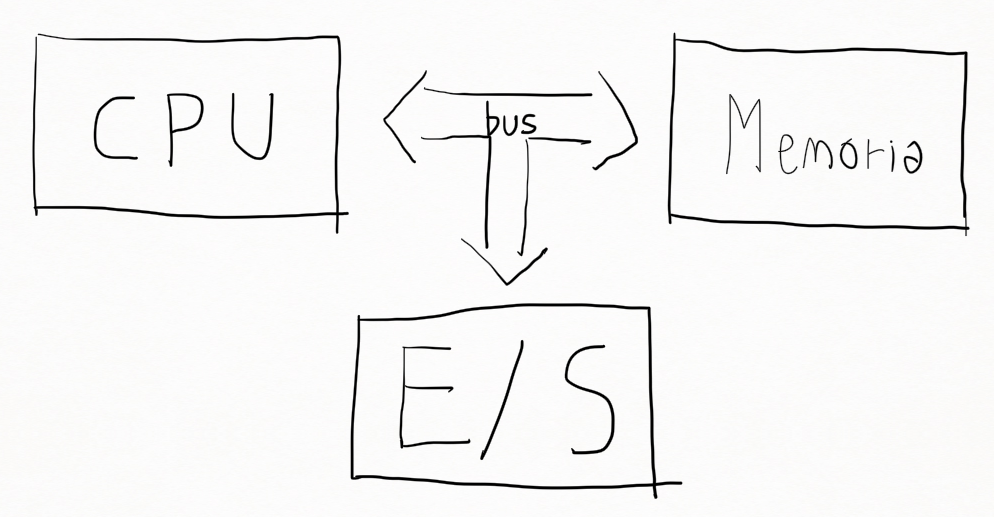
\includegraphics[scale=0.3]{ArqVN.png}
	\caption{Esquema de los componentes de la arquitectura de Von Neumann.}
	\label{fig-ArqVN}
\end{figure}

El procesador tiene tres componentes que cumplen distintas funciones: la unidad de control, la unidad aritmética lógica (ALU) y el banco de registros. La unidad aritmética lógica consta de varios circuitos combinatorios que implementan operaciones básicas, como por ejemplo operaciones lógicas como <<y>>, <<o>> y <<no>>, operaciones aritméticas como suma y multiplicación (para números codificado con una cantidad fija de bits) u operaciones básicas sobre cadenas e bits, como el {\sl shift}, que traslada cada bit un lugar a la derecha o la izquierda. El banco de registros consta de ciertos registros (un tipo de circuito que almacena valores) en general variables que se usan para el funcionamiento de la CPU. Por ejemplo, pueden tener los argumentos de las operaciones que va a realizar la unidad aritmética lógica. También hay un registro de particular importancia llamado {\sl program counter}, que indica la posición de memoria de la siguiente instrucción a ejecutar (es de suma importancia, ya que la idea del CPU es ejecutar secuencias de instrucciones). Finalmente, la unidad de control es un circuito secuencial que se encarga de llevar a cabo las instrucciones, usando la unidad aritmética lógica y el banco de registros. Estos circuitos secuenciales están hechos para que automáticamente se lea e identifique la instrucción que indica el program counter, se carguen nuevos datos en los registros (si es necesario), se realice la operación indicada en la ALU y se guarde el resultado donde corresponda (si hay que hacer alguna operación), y que el program counter avance a la siguiente instrucción, para poder repetir el proceso.

Respecto a la suma, la ALU al ser un circuito combinatorio, es en realidad como una tabla que tiene el resultado para cada combinación de operandos. Las sumas que se realizan directamente por la ALU pueden ser por ejemplo de números representados por uno o dos bytes (donde un byte es por definición una secuencia de 8 bits). Como la cantidad de números representables crece exponencialmente con la cantidad de bits, hacer sumas de números más grandes por la ALU (que lo que hace es tener una tabla con todos los resultados) es extremadamente ineficiente. Lo que se hace para realizar sumas con números más grandes es descomponerlas como una secuencia de instrucciones más sencillas. Esto es como lo que se hace en los algoritmos aritméticos básicos. Pensemos por ejemplo en el producto. Está la tabla de multiplicación que uno se aprende de memoria (lo cual es análogo a lo que está en los circuitos de la ALU) pero luego a partir de eso, siguiendo un algoritmo (secuencia de instrucciones) se puede calcular la multiplicación de números de cualquier cantidad de cifras sin precisar saber nada más de memoria.

La memoria es un dispositivo electrónico capaz de almacenar muchos valores, los cuales pueden ser leídos o modificados. Tiene la estructura de un gran vector de bytes, indizado por secuencias de bits de largo fijo. Por ejemplo, si se usan dos bits para indizar, los lugares de la memoria serían el {\tt 00}, el {\tt 01}, el {\tt 10} y el {\tt 11}, cada uno de los cuales contendría un byte de información. En las computadoras actuales la memoria suele tener del orden de $2^{32}$ lugares de memoria, es decir 4GB ($2^{10}$ bytes es un KB, $2^{20}$ es un MB y $2^{30}$ es un GB). Se trata de la llamada memoria RAM. Actualmente la cantidad de bits que se usa para indizar es 64 (la llamada arquitectura de 64 bits), pero eso no implica que todas las palabras que se puedan formar correspondan a direcciones válidas (en computadoras personales no existe actualmente memoria de $2^{64}$ bytes, que serían como 16 mil millones de gigabytes). Conceptualmente el banco de registros del procesador es como una memoria. El motivo de que existan las dos cosas es que el banco de registros es memoria de mejor calidad y más cara que se reserva para estar dentro de la CPU, mientras que la memoria RAM es más lenta pero más económica para tener en grandes cantidades.

\subsection{Ejemplo de programa}

Hagamos un ejemplo del funcionamiento de una computadora. Supongamos que tenemos 8 registros (enumerados) de un byte cada uno y que las direcciones de memoria son indizadas también por un byte. Supongamos que tenemos las siguientes instrucciones
\begin{itemize}
	\item {\tt LOAD}. Instrucción con dos parámetros: {\tt M} y {\tt R}, que lo que hace es cargar en el registro {\tt R} el contenido de la dirección de memoria {\tt M}.
	\item {\tt SAVE}. Instrucción con dos parámetros: {\tt M} y {\tt R}, que lo que hace es guardar en la dirección de memoria {\tt M} el contenido del registro {\tt R}.
	\item {\tt ADD}. Instrucción con tres parámetros: $\mathtt{R_1}$, $\mathtt{R_2}$ y $\mathtt{R_3}$ que lo que hace es sumar el contenido de los registros $\mathtt{R_1}$ y $\mathtt{R_2}$ y guardar el resultado en el registro $\mathtt{R_3}$.
\end{itemize}


Respecto a la operación {\tt ADD}, como los contenidos de los registros son bytes, o sea 8 bits, se considera que cada secuencia de 8 bits representa en binario un número entre $0$ y $2^8-1$. En caso de que el resultado se salga del rango, se le sustraye $2^8$ al resultado (formalmente, es la suma de $\mathbb{Z}_{2^8}$, es decir aritmética modular).

Por otra parte, cada instrucción está codificada por un byte. Supongamos que el código de {\tt LOAD} es {\tt 00000001}, el de {\tt SAVE} es {\tt 00000010} y el de {\tt ADD} es {\tt 00000011}.

Asumamos también que los tres primeros registros, $\mathtt{R_1}$, $\mathtt{R_2}$ y $\mathtt{R_3}$ se identifican con los bytes {\tt 00000001}, {\tt 00000010} y {\tt 00000011}.

Supongamos que queremos un programa que lo que haga es sumar los contenidos de las direcciones de memoria {\tt 10000001} y {\tt 10000010} y guardar el resultado en la dirercción {\tt 10000011}. Podríamos hacerlo realizando cuatro instrucciones. Primero un {\tt LOAD} para cargar el contenido de la primera dirección de memoria en el registro 1, luego otro {\tt LOAD} para cargar el contenido de la segunda dirección de memoria en el registro 2, luego un {\tt ADD} para sumar los contenidos de los registros 1 y 2 y guardar el resultado en el registro 3 y finalmente una {\tt SAVE} para guardar el contenido del registro 3 en la tercera dirección de memoria. Primero escribamos las instrucciones de un modo un poco más abstracto (para no ir de una a los 0s y 1s).  Definamos las direcciones de memoria {\tt 10000001}, {\tt 10000010} y {\tt 10000011} como $\mathtt{M_1}$, $\mathtt{M_2}$ y $\mathtt{M_3}$, respectivamente. El programa sería lo siguiente.
\begin{align*}
	&\mathtt{LOAD} \quad\mathtt{M_1~R_1}\\
	&\mathtt{LOAD}  \quad\mathtt{M_2~R_2}\\
	&\mathtt{ADD}  \quad\mathtt{R_1~R_2~R_3}\\
	&\mathtt{SAVE}  \quad\mathtt{M_3~R_3}
\end{align*} 
Esto último es lo que se considera como un programa escrito en {\sl assembler}. Es una forma de programar en la que cada línea es una instrucción del procesador, pero se pueden usar los nombres de las instrucciones y nombres de lugares de memoria, en lugar de tener que escribir todo en bits. El mismo programa escrito ahora en código máquina, es decir en bits, exactamente como iría en la memoria, sería:
\begin{align*}
	&\mathtt{00000001} \quad\mathtt{10000001~00000001}\\
	&\mathtt{00000001}  \quad\mathtt{10000010~00000010}\\
	&\mathtt{00000011}  \quad\mathtt{00000001~00000010~00000011}\\
	&\mathtt{00000010}  \quad\mathtt{10000011~00000011}
\end{align*}
La organización en líneas del código es para que sea más fácil de leer, pero el programa de hecho es simplemente 0000000110000001000000010000000110000010000000100000001100 0000010000001000000011000000101000001100000011. Si tenemos en alguna parte de la memoria esa secuencia de bytes y el program counter indicando la dirección donde comienza, la computadora automáticamente lo ejecutará. Esto se ilustra en la figura \ref{fig-ArqVNEjProg}.

Cabe resaltar que este es un ejemplo muy sencillo. Hay otros tipos de instrucciones (por ejemplo las que modifican el program counter y permiten realizar ciclos) y los programas suelen ser mucho más largos. De hecho, cuales son exactamente las instrucciones y cómo se codifican varía de un procesador a otro.

\begin{figure}
	\centering
	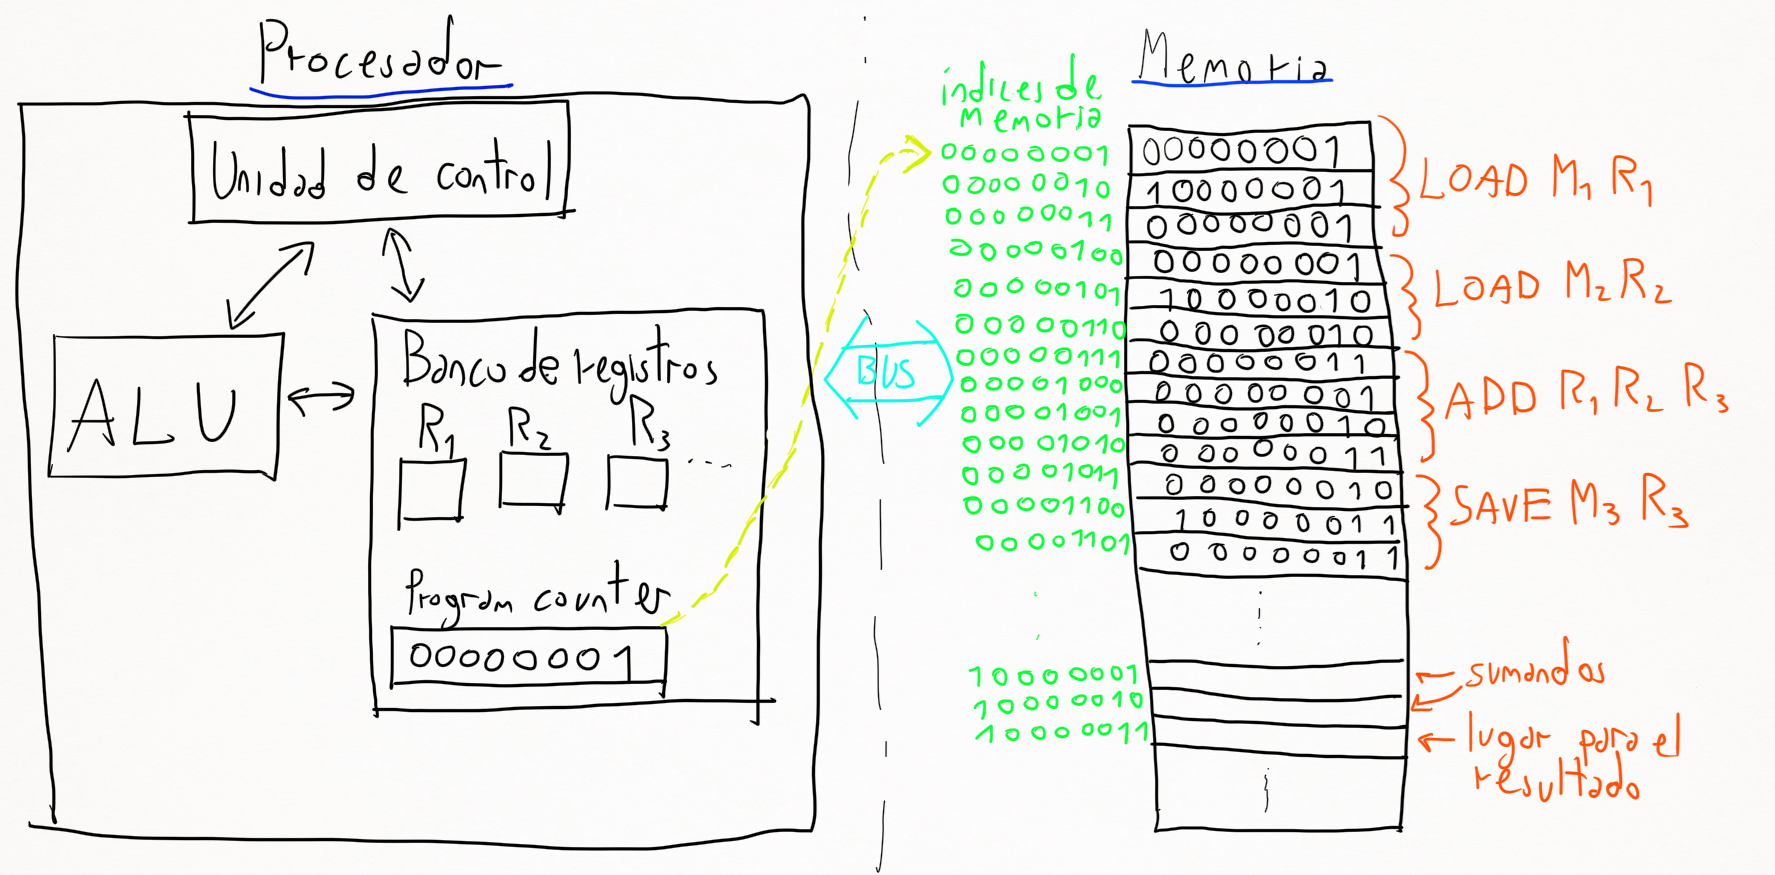
\includegraphics[scale=0.33]{ArqVNEjProg.png}
	\caption{Esquema de una computadora con un programa.}
	\label{fig-ArqVNEjProg}
\end{figure}

\section{Lenguajes de programación y compiladores}

Dada una computadora que sigue la arquitectura de Von Neumann, se puede implementar cualquier función computable con algún programa escrito en código máquina. Sin embargo, hay algunas características poco prácticas.
\begin{itemize}
	\item Es relativamente difícil escribir programas como secuencias de instrucciones de máquina. En general hay muchos más detalles que entran en juego que en el ejemplo dado y hace falta mucho esfuerzo para escribir programas que hagan operaciones complejas.
	\item Distintos procesadores suelen tener distintas instrucciones. Además, incluso cuando la instrucción es la misma puede estar codificada distinto. Por ejemplo, puede que en un procesador {\tt 00000001} sea el código de la suma y en otro sea el código de la operación de cargar en un registro. Por lo tanto, un programa que se escribe para un procesador probablemente no funcione en otro.
\end{itemize}
Estos factores dificultan escribir programas y hacen que solamente lo puedan hacer especialistas. Sin embargo, con el tiempo se desarrolló un concepto que mejora la situación, haciendo que sea más fácil desarrollar un programa y que la curva de aprendizaje sea más corta. Se trata de los {\bf lenguajes de programación}.

Los lenguajes de programación introducen abstracciones que permiten escribir programas sin preocuparse por detalles técnicos de cómo se resuelve con instrucciones del procesador. Por ejemplo, se introduce el concepto de las variables para trabajar con datos sin preocuparse por en qué direcciones de memoria están ni de cómo se utilizan los registros para operaciones. Por ejemplo, se si tenemos tres variables {\tt x, y} y {\tt z}, para sumar los contenidos de las primeras dos y guardarlo en la tarcera, simplemente habría que escribir:
$$\mathtt{z} = \mathtt{x}+\mathtt{y}
$$
sin preocuparse ni por en qué dirección va cada una ni de si hay que usar registros para realizar la suma o no.

Un programa escrito en un lenguaje de programación es un archivo de texto. Se compone por líneas escritas con caracteres comunes que representan operaciones de forma clara (para una persona). Las instrucciones escritas en un lenguaje de programación no pueden ser ejecutadas directamente por un procesador (estos solo entienden ceros y unos). En este punto entran en juego los {\bf compiladores}. Estos son programas cuya función es traducir un programa escrito en un lenguaje de programación a un programa en código máquina. Se los puede pensar como funciones cuya entrada es un programa escrito en un lenguaje de programación y su salida es una secuencia de instrucciones de procesador (lenguaje máquina) que hace lo mismo. El proceso usual al programar es el siguiente: primero se escribe el programa en un lenguaje de programación, luego se usa un compilador para traducirlo a código de máquina y finalmente se lo ejecuta.

Los lenguajes de programación junto con los compiladores solucionan las dos desventajas previamente mencionadas. Por una parte, escribir en un lenguaje de programación es más fácil que en lenguaje máquina. Por otra parte, un lenguaje de programación suele tener compiladores para distintos procesadores, de modo que un mismo programa escrito en este lenguaje puede ser compilado a código máquina de distintos procesadores y por lo tanto ser ejecutado en cada uno de ellos.

Se dice que un lenguaje de programación es de alto o bajo nivel según el nivel de abstracción que hay por sobre el lenguaje de máquina (instrucciones del procesador). Escribir directamente las instrucciones del procesador o código en assembler es de bajo nivel, mientras que usar un lenguaje de programación que incluye abstracciones como variables, estructuras de datos o iteraciones es de alto nivel. Entre los distintos lenguajes de programación hay varios niveles de abstracción.


El lenguaje {\tt c} (así como {\tt pascal}) es un lenguaje de relativamente bajo nivel, pues tiene abstracciones como las previamente mencionadas, pero no está {\sl tan} lejos del lenguaje máquina. Mirando un programa escrito en {\tt c}, para alguien con experiencia no es tan difícil darse cuenta de cómo podrían ser las instrucciones en lenguaje máquina.

Por otra parte, el lenguaje {\tt python}, que es el que usaremos en el curso, es de muy alto nivel. Esto significa que tiene abstracciones muy complejas por sobre el lenguaje máquina, las cuales hacen que se pueda programar en base a razonamientos intuitivos sin saber cómo se haría en lenguaje de máquina. De hecho puede ocurrir que una sola línea de código en {\tt python} corresponda a cientos de instrucciones del procesador, con lo que se resuelven automáticamente detalles técnicos y se le ahorra trabajo al programador. En general usar un lenguaje de programación de alto nivel es más fácil que usar uno de bajo nivel. La desventaja que tienen es que las abstracciones pueden hacer que el programa no sea lo más eficiente posible. En general un programa escrito en {\tt c} es mucho más rápido que uno equivalente en {\tt python} (pero mucho más difícil de escribir).

\chapter{Programación en python}

En este capítulo se presentan los conceptos básicos para programar en el lenguaje python. Si bien se trata de un lenguaje específico, los conceptos se aplican de forma muy similar en otros. El objetivo de este material es presentar los elementos de forma conceptual. Para asimilarlos bien se recomienda complementar con otros materiales que incluyan más ejemplos y además escribir y ejecutar código uno mismo (para instalación y ejecución ver sección \ref{sec-instalyEjec}).

Respecto a materiales que incluyen ejemplos, se recomienda el tutorial de la documentación oficial de python: \href{https://docs.python.org/es/3.13/tutorial/index.html}{https://docs.python.org/es/3.13/tutorial/index.html}. Ese tutorial contiene mucho más que lo que se necesita para el curso. Se recomienda ver todo el capítulo 3 y algunos conceptos del 4 para ver ejemplos, pero sin preocuparse por detalles técnicos (hay explicaciones pensadas para gente que ya conoce conceptos de programación por otros lenguajes).

Cabe aclarar que lo que se ve en este curso es solo una pequeña introducción a python. Además, las explicaciones buscan transmitir ideas del lenguaje, sin necesariamente ser totalmente correcto con las definiciones formales de los conceptos o exactamente cómo funciona por dentro. Para esto se recomienda nuevamente la documentación (reiterando que excede los contenidos del curso).

\section{Instalación y ejecución}\label{sec-instalyEjec}

Instalar python es principalmente instalar el compilador que traduce el código en python a lenguaje máquina, de modo que podamos ejecutar lo que programemos. Un detalle técnico es que en lugar de llamársele <<compilador>> se le llama <<intérprete>>. Esto es porque en lugar de pasar todo el programa a lenguaje máquina y luego ejecutarlo, va pasando las líneas de código a lenguaje máquina una por una a la vez que se van ejecutando. Se dice que es un compilador cuando primero se traduce todo a lenguaje máquina y luego se lo ejecuta.

En el sistema operativo linux, en general python ya viene instalado por defecto. Por otra parte, en windows no es el caso (nos enfocaremos en este sistema operativo, ya que quienes utilizan linux es más probable que ya sepan ejecutar python). Una forma de instalarlo es descargando el instalador desde el sitio web de python y ejecutándolo (\href{https://www.python.org/downloads/}{https://www.python.org/downloads/}). Durante la instalación es importante marcar la opción de <<Add python.exe to PATH>> (figura \ref{fig-InstallPython}), por motivos que vermos a contiuación.

\begin{figure}
	\centering
	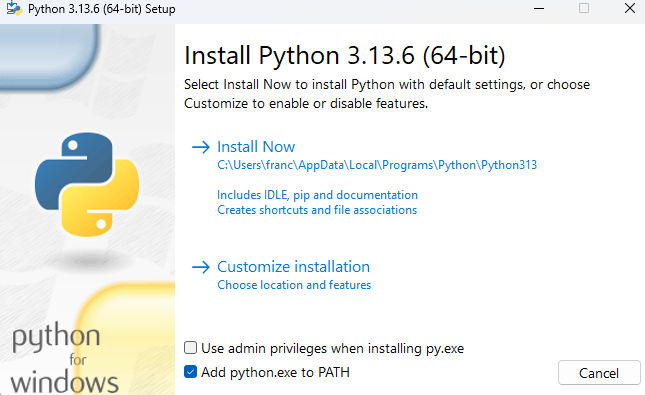
\includegraphics[scale=0.5]{InstallPython.png}
	\caption{Es importante marcar la opción <<Add python.exe to PATH>>.}
	\label{fig-InstallPython}
\end{figure}

Vamos a ejecutar python desde una ventana de comandos (o terminal). Esto es una ventana a través de la cual se le escriben comandos al sistema operativo. En windows se llama Windows PowerShell o símbolo del sistema.

Si hicimos bien la instalación de python, al abrir una ventana de comandos, si se escribe python y se toca enter, comienza a ejecutarse el intérprete, el cual nos permite ir ingresando instrucciones una a una. Los tres símbolos de >~significan que el intérprete está listo para recibir instrucciones. Una primera cosa que se puede hacer es usarlo como calculadora, escribiendo expresiones aritméticas y tocando enter (figura \ref{fig-cmdPython}). Para salir del intérprete se puede escribir {\tt quit()} y tocar enter.

Al escribir python, lo que se hace es ejecutar el intérprete. Para que esto funcione, el sistema operativo debe tener la dirección en la que python está instalado dentro de una cierta lista. Esto es lo que se hace al marcar la opción <<Add python.exe to PATH>> durante la instlación. Luego de haber ejecutado python en la ventana de comandos, el uso del intérprete ocurre dentro de esta misma ventana, sin usarse ninguna interfaz gráfica (a diferencia de la mayoría de los programas que utilizamos). En general no hay necesidad de nada más sofisticado.

\begin{figure}
	\centering
	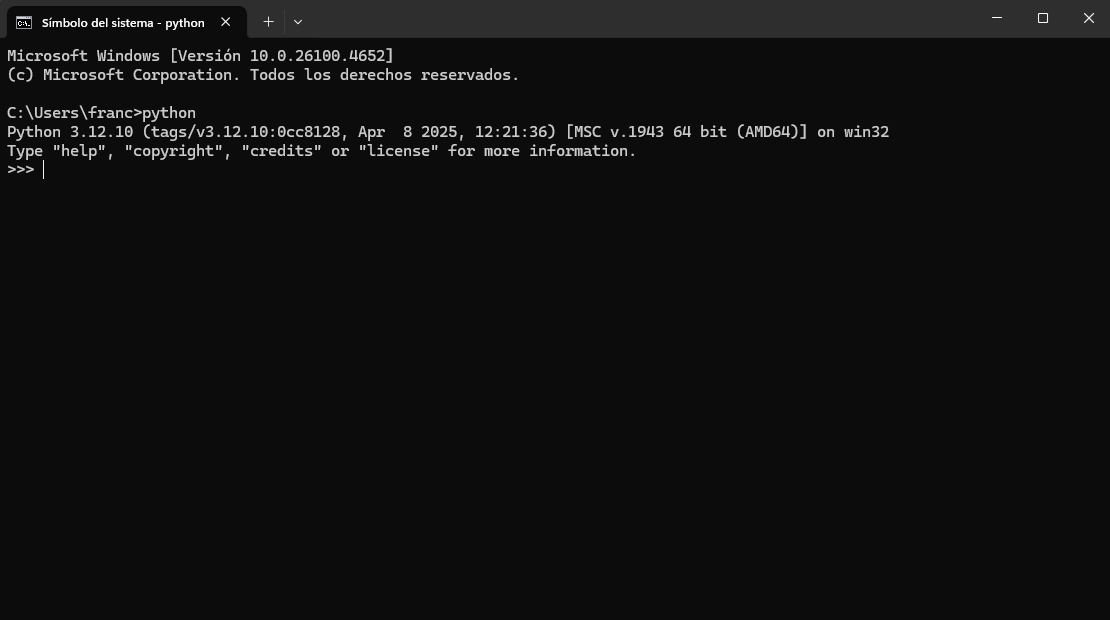
\includegraphics[scale=0.5]{cmdPython.png}
	\caption{Ventana de comandos con el intérprete de python.}
	\label{fig-cmdPython}
\end{figure}

Con la modalidad de uso del intérprete que vimos, se escriben y ejecutan lineas una a una. Por otra parte, se puede escribir un archivo con varias lineas de código y pasárselo al intérprete para que lo ejecute. El código se escribe en un archivo de formato <<.py>>. Para escribir este tipo de archivos se puede usar cualquier editor de texto, pero se recomienda utilizar un editor de código especializado. Uno muy popular actualmente es visual studio code (\href{https://code.visualstudio.com/}{https://code.visualstudio.com/}). Una vez que se escribió el archivo con el código y se lo tiene guardado en una carpeta, hay que abrir una ventana de comandos en esa carpeta (cada ventana de comandos trabaja en alguna carpeta particular) e ingresar <<python>> seguido del nombre del archivo con el <<.py>> incluido. Esto se ejemplifica en la figura \ref{fig-ejecPython}.

Para todo lo que mencionamos en esta sección, buscando en internet (motores de búsqueda como google, o sitios con contenido audiovisual como youtube) se encuentran muchos tutoriales. 

\begin{figure}
	\centering
	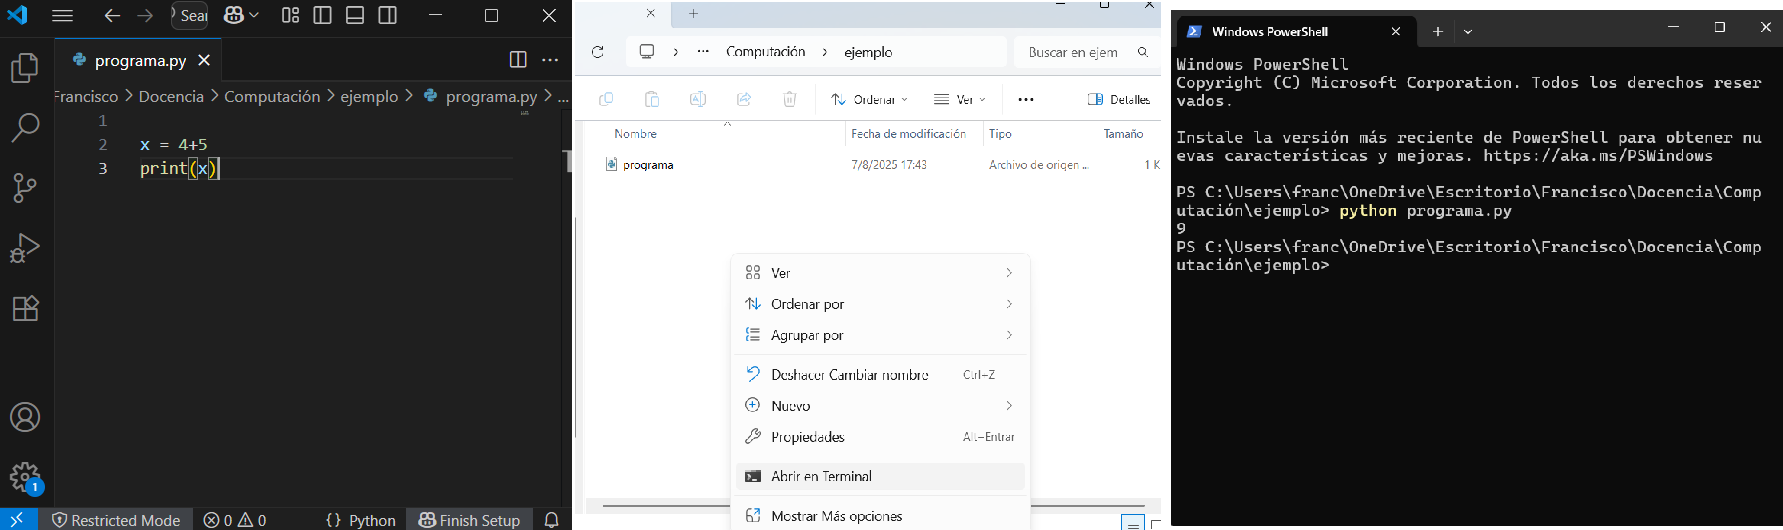
\includegraphics[scale=0.4]{ejecPython.png}
	\caption{A la izquierda visual studio code con el código del archivo llamado programa.py. Al centro se ve la carpeta llamada ejemplo en la que está el archivo. Dentro de esa carpeta se abre la terminal. A la derecha se ve la terminal en la que se escrie <<python programa.py>>. Antes del símbolo >, a la izquierda de <<python>>, se indica la carpeta en la que está la terminal. Si al hacer click derecho en la carpeta no aparece la opción <<abrir en terminal>>, puede aparecer al hacer click derecho manteniendo apretado mayus/shift (recordar que powershell también es una terminal). En todo caso, para problemas como este se recomienda buscar en internet, con lo cual se suele encontrar alguna solución rápidamente. También se puede abrir una terminal en cualquier sitio y cambiar la ubicación con instrucciones específicas, como {\tt cd} (buscar en internet en caso de que haya interés).}
	\label{fig-ejecPython}
\end{figure}
\section{Tipos de datos}

Una de las abstracciones que aportan los lenguajes de programación consiste en los tipos de datos. Se trata de la abstracción de distintos tipos de objetos, como enteros, texto o listas, cada uno de los cuales tiene distintos posibles valores y distintas operaciones que se pueden aplicar. Por supuesto que todos estos objetos se codifican como secuencias de bits, pero poder trabajar pensando en términos de objetos de distinto tipo hace que programar sea más intuitivo. Se puede saber el tipo de datos de un objeto escribiendo {\tt type()} con el objeto entre paréntesis. Veamos algunos de los tipos de datos que tiene python con algunas de las operaciones disponibles. 

\subsection{Booleanos}

Los booleanos conforman un tipo de datos que representa valores de verdad. Tiene solo dos objetos: {\tt True} y {\tt False}. Se tienen las operaciones lógicas básicas: {\tt not}, {\tt and} y {\tt or}. Hay algunos ejemplos en la figura \ref{fig-ejemploBool}. Si aplicamos {\tt type()} a un boolano, retorna {\tt class bool}. En general los booleanos por sí solos no suelen ser de mucha utilidad. Su principal aplicación es en condicionales e iteraciones, que estudiaremos en lo siguiente. 

\begin{figure}
	\centering
	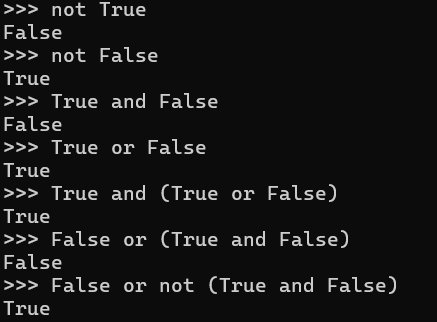
\includegraphics[scale=0.6]{ejemploBool.png}
	\caption{Ejemplos de operaciones con booleanos.}
	\label{fig-ejemploBool}
\end{figure}

\subsection{Enteros}

Se trata de un tipo de datos para representar enteros naturales. Los objetos son {\tt 0}, {\tt 1} {\tt -1}, {\tt 2}, {\tt -2}, etc. Si aplicamos {\tt type()} a un boolano, retorna {\tt class int} por {\sl integer}. Tienen las operaciones aritméticas elementales, que se muestran en la figura \ref{fig-ejemploInt}. Notar que la división entera es con dos barras. Una barra sola es otra operación que veremos en la brevedad. Por otra parte se tienen las operaciones de comparación, que reciben dos enteros y retornan un booleano. Se muestran en la figura \ref{fig-ejemploComp}. En el caso de la igualdad, si se escribe un solo símbolo <<=>> es una asignación, lo cual veremos más adelante.

\begin{figure}
	\centering
	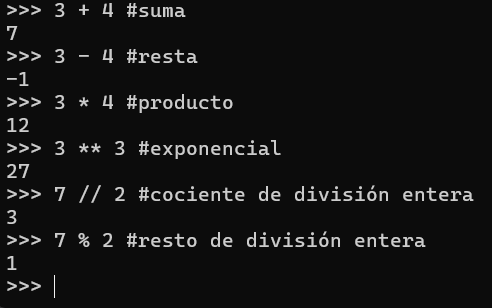
\includegraphics[scale=0.6]{ejemploInt.png}
	\caption{Operaciones aritméticas básicas. Lo que está escrito después de los \# son comentarios. Los comentarios son ignorados por el intérprete, la función que cumplen es de aclaraciones para personas que lo leen.}
	\label{fig-ejemploInt}
\end{figure}

\begin{figure}
	\centering
	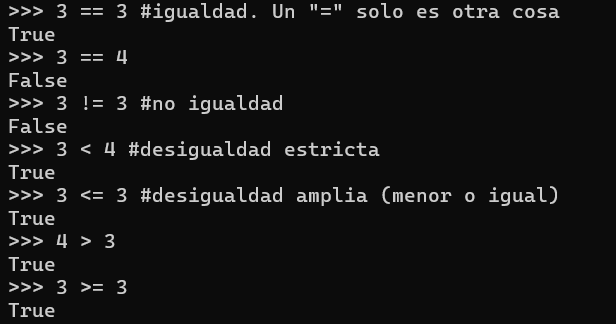
\includegraphics[scale=0.6]{ejemploComp.png}
	\caption{Comparaciones entre enteros. }
	\label{fig-ejemploComp}
\end{figure}

\subsection{Números de punto flotante}

Se trata de una representación para operar con números reales usando información finita. De hecho lo que representan es un conjunto finito de números racionales, pero a menos de cierta aproximación se opera con ellos igual que con números reales. Estos números se escriben con la notación usual para números con parte fraccionaria o con notación científica, en ambos casos separando la parte fraccionaria con un punto. Están las mismas operaciones aritméticas y comparaciones, salvo por la división. En punto flotante tenemos el operador / para la división de números reales. Un detalle importante es que si aplicamos la operación / a enteros, el resultado es de punto flotante, independientemente de que la división de exacta o no. Se presentan ejemplos en la figura \ref{fig-ejemploFloat}.

Los números de punto flotante tienen limitaciones debido al hecho de que se pueden representar solo finitos números. Por ejemplo, si a {\tt 1.0} le sumamos un número muy chico, se redondea a {\tt 1.0}, lo cual puede ser problemático en algunas situaciones. Ignoraremos este problema, pero es un tema relevante dentro del área de análisis numérico.

Hay más operaciones sobre punto flotante que se pueden realizar si importamos la biblioteca {\tt math}. Más adelante en el curso nos centraremos más en las bibliotecas, pero por ahora alcanza con saber que es algo que permite extender el lenguaje con más operaciones. Para incluir el contenido de la biblioteca {\tt math} hay que escribir la instrucción {\tt import math}. Después de eso se pueden utilizar las operaciones incluidas en esta biblioteca. Esto se hace escribiendo el nombre de la biblioteca, un punto y el nombre de la operación. Por ejemplo, tiene una operación de raiz cuadrada que se utiliza escribiendo {\tt math.sqrt()}, donde al argumento lo ponemos entre los paréntesis. Por otra parte, está la operación {\tt math.floor()} que retorna el entero más cercano a la izquierda. Esta última función retorna efectivamente un objeto de tipo entero y no un objeto de tipo punto flotante con valor entero. Se presentan ejemplos en la figura \ref{fig-ejemploMath}.

En general se pueden realizar operaciones aritméticas entre enteros y números de punto flotante. En ese caso, el resultado es de punto flotante. Lo que ocurre en estos casos es que (al menos conceptualmente) se convierten automáticamente enteros a punto flotante. Al aplicar / a enteros ocurre lo mismo (al menos conceptualmente): primero los enteros se transforman a punto flotante y luego se aplica la operación. Por otra parte, en general no hay conversión automática de punto flotante a entero, aunque el número no tenga parte fraccionaria.

\begin{figure}
	\centering
	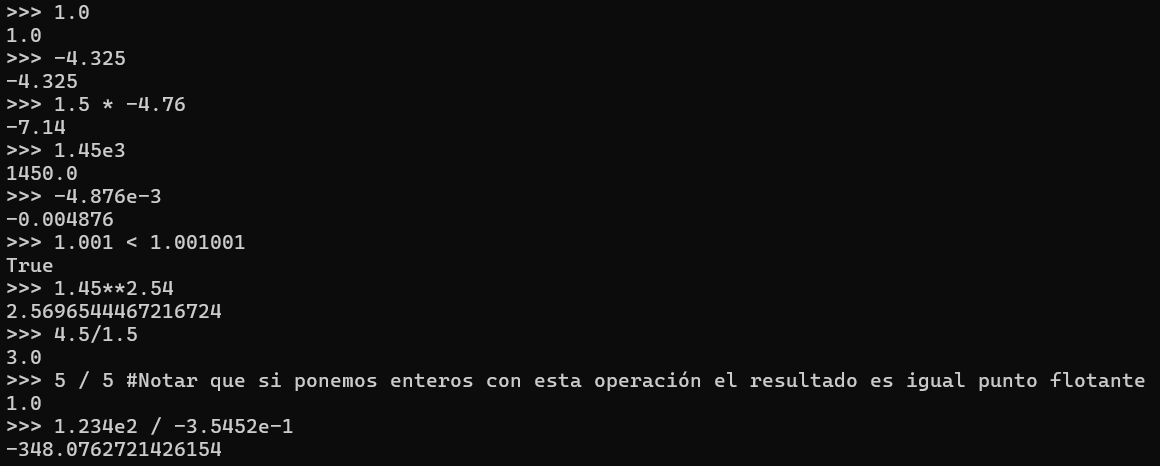
\includegraphics[scale=0.6]{ejemploFloat.png}
	\caption{Ejemplos de números de punto flotante.}
	\label{fig-ejemploFloat}
\end{figure}

\begin{figure}
	\centering
	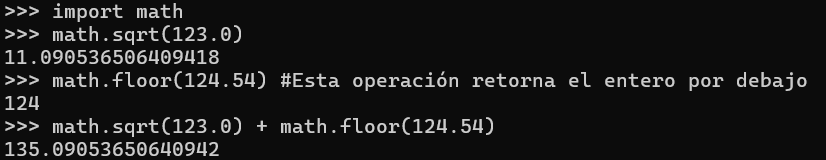
\includegraphics[scale=0.6]{ejemploMath.png}
	\caption{Ejemplos de operaciones de la biblioteca math.}
	\label{fig-ejemploMath}
\end{figure}


\subsection{Texto}

En python se puede representar texto, es decir, secuencias de caracteres. Esto se hace delimitando con comillas simples o dobles. En general se les llama {\sl strings} y de hecho {\tt type()} retorna {\tt class str}. Algunos ejemplos son ``Hola.'', ``345'', `` '' (espacio)  y ``'' (string vacío). No hay que confundir, por ejemplo, al string ``345'' con el entero {\tt 345}, pues son objetos de distintos tipos (se lo puede verificar con {\tt type()}). Con el símbolo + se realiza la operación de concatenación, es decir ``Hola.'' + ``345'' da ``Hola.325''. Notar que el símbolo + tiene varios usos. Cual de todos se usa depende del tipo de los argumentos. Por ejemplo, {\tt 12 + 12} da {\tt 24} (los argumentos son enteros, por lo que se los suma), mientras que {\tt ``12'' + ``12''} da {\tt ``1212''} (los argumentos son strings, por lo que se los concatena).

\subsection{Listas}

Las listas conforman un tipo de datos compuesto. Cada lista es, como su nombre sugiere, una lista de objetos. Una lista se comienza y se termina con <<[>> y <<]>>. Los distintos elementos se separan con comas. Por ejemplo: {\tt[0,1,4]}, {\tt[``aa'',``a'',``'']}, {\tt [3.5, ``a'']} y {\tt[]}. Las listas pueden tener cualquier cantidad de elementos (a partir de cero) y estos elementos pueden ser de cualquier tipo, incluso otras listas. Por ejemplo {\tt [[],[]]} es una lista con dos elementos, que los dos son la lista vacía. Con + se puede concatenar listas, de modo que {\tt [[],[]] + [1]} da {\tt [[],[],1]}.


\section{Variables y asignaciones}

Las variables son abstracciones que consisten en un nombre que se puede usar para referenciar objetos de distintos tipos de datos. Se puede pensar que el objeto referenciado por la variable es su valor. Nombres válidos de variable son secuencias de caracteres alfanuméricos y <<\_>> en los que el primer carácter no es un número, como por ejemplo {\tt x, x1, total} y {\tt altura\_caja}.

La asignación es la instrucción básica de python para dar un nuevo valor a una variable. La sintaxis es:
$$\mathtt{var}~=~\mathtt{expr}$$
donde $\mathtt{var}$ es el nombre de la variable a la que queremos asignar un objeto (es decir, hacer que la variable referencia al objeto) y $\mathtt{expr}$ es una expresión que determina el objeto a asignar.  Es distinto al uso que se le da al símbolo <<$=$>> en matemáticas (en particular, los lados tienen roles distintos), asemejándose más al de <<$:=$>>. La expresión puede ser un objeto fijo, una variable o algo más elaborado, por ejemplo con operaciones. Incluso puede contener la misma variable {\tt var}. En ese caso para evaluar la la expresión se usa el valor actual de la variable y luego se le asigna el resultado. Si en la expresión ponemos alguna variable aún no definida, se produce un error. Los siguientes son algunos ejemplos.

\begin{verbatim}
>>> x = 10
>>> x #Mostrar el valor de la variable x
10
>>> x = 10 #asignamos el valor 10 a la variable x
>>> x #Mostrar el valor actual de la variable x
10
>>> x*2
20
>>> x1 = x**2
>>> x1
100
>>> x = x + 1
>>> x
11
>>> z = 20
>>> z = z + x2 #Usamos una variable x2 que no definimos antes. Da error
Traceback (most recent call last):
File "<stdin>", line 1, in <module>
NameError: name 'x2' is not defined. Did you mean: 'x'?
>>> lista1 = ["a","b","c"]
>>> lista2 = [1,2,3]
>>> lista3 = lista1 + lista2
>>> lista3
['a', 'b', 'c', 1, 2, 3]
\end{verbatim}
En python las variables no guardan un valor dentro de ellas, sino que en realidad referencian a un objeto que está fuera en otro lado. Esto es un detalle técnico al que volveremos en la sección \ref{sec-memoriaCompartida}.
\section{Indizado y slicing}

El indizado se trata de cómo acceder a elementos de ciertos lugares en estructuras de datos compuestas. Vamos a introducirlo para listas y strings (aunque pensando los strings como listas de caracteres es muy análogo).

Dada una variable {\tt x} que tiene una lista y un entero $n$ (o una variable que contiene al entero $n$), tenemos que {\tt x[$n$]} es el elemento número $n$ de la lista. En caso de que {\tt x} contenga un string, es el carácter número~$n$. En python (así como en la mayoría de los lenguajes de programación) la enumeración comienza en 0. Por lo tanto, dada una lista {\tt x}, su primer elemento es {\tt x[0]}. Lo mismo se puede aplicar con strings, caso en el que se retorna un substring formado solamente por el caracter del lugar $n$.

Tanto para listas como para strings, si el índice se pasa del último elemento, se produce un error. En python se puede usar la función {\tt len()} para determinar el largo de una lista o un string. Los índices válidos de {\tt x} van desde {\tt 0} hasta {\tt len(x)-1}.

Por otra parte, el {\sl slicing} consiste en indizar por rangos, obteniéndose sublistas o substrings. La versión más sencilla, dada una lista {\tt x} y dos enteros $n,m$, es {\tt x[$n:m$]}, que resulta en la sublista de todos los elementos con índice $i$ tal que $n\leq i < m$. Notar que el extremo de abajo usa orden inclusivo y el de arriba estricto. En este caso no hay problemas si nos pasamos del último elemento. El resultado puede ser la lista vacía o el string vacío.

También se pueden hacer asignaciones a elementos de cierto índice, permitiendo modificar el valor de cierto lugar de una lista. Con strings no se permite hacer esto.

Veamos ejemplos de todo lo anterior.
\begin{verbatim}
>>> x = [1,2,3,4,5]
>>> s = "Hola 1."
>>> x[0]
1
>>> s[1]
'o'
>>> s[4] #Va a retornar un espacio
' '
>>> len(s)
7
>>> s[6]
'.'
>>> s[7]
Traceback (most recent call last):
File "<stdin>", line 1, in <module>
IndexError: string index out of range
>>> x[5]
Traceback (most recent call last):
File "<stdin>", line 1, in <module>
IndexError: list index out of range
>>> x[0:2]
[1, 2]
>>> x[2:5]
[3, 4, 5]
>>> x[2:10]
[3, 4, 5]
>>> x[6:10]
[]
>>> x[1]=40
>>> x
[1, 40, 3, 4, 5]
\end{verbatim}

Con listas de listas se puede concatenar indizados. Es decir, si {\tt l} es una lista cuyos elementos son listas, {\tt l[i][j]} es el {\tt j}ésimo elemento de la {\tt i}ésima lista. Los paréntesis implícitos van de la siguiente forma: {\tt (l[i])[j]}, pues {\tt l[i]} es una lista a la cual se aplica el índice {\tt j}. A modo de ejemplo:
\begin{verbatim}
>>> l = [[1,2],[3,4],[5,6]]
>>> len(l) #Tiene 3 elementos que son las listas de adentro
3
>>> l[0] # Retorna la primera lista
[1, 2]
>>> l[1] # Retorna la segunda lista
[3, 4]
>>> l[2] # Retorna la tercera lista
[5, 6]
>>> l[3] # Produzcamos un error de índice
Traceback (most recent call last):
File "<stdin>", line 1, in <module>
IndexError: list index out of range
>>> len(l[0]) #Largo de la lista [1,2]
2
>>> l[0][0] #Elemento 0 de lista 0
1
>>> l[0][1] #Elemento 1 de lista 0
2
>>> l[1][0] #Elemento 0 de lista 1
3
\end{verbatim}
En general de hecho, en caso de que {\tt l[i]} sea una lista, se puede hacer con ella lo mismo que con una lista que esté dada por una variable. Por ejemplo, también se puede hacer slicing con {\tt l[i][n:m]}, lo cual dará la sublista de {\tt l[i]} correspondiente, o determinar su largo con {\tt len(l[i])}.
\subsection{Referencias múltiples}\label{sec-memoriaCompartida}

Vamos a tratar un detalle un poco técnico. La mayoría de las veces no es relevante, pero a veces puede ser fuente de errores inesperados.

Recordar que las variables no contienen los objetos, sino que los referencian. Esto es particularmente importante con listas porque estas se pueden modificar, entonces si dos variables referencian la misma lista y desde una la modificamos, esto se reflejará en la otra variable. Veamos un ejemplo.
\begin{verbatim}
>>> l1 = [1,2,3]
>>> l2 = l1
>>> l2[0] = 0
>>> l1
[0, 2, 3]
\end{verbatim}
Esto ocurrió porque la asignación {\tt l2=l1} lo que hizo es que la variable {\tt l2} referencie la misma lista que {\tt l1}. Para que la lista de {\tt l2} sea una lista distinta a la de {\tt l1} pero con los mismos valores, habría que escribir {\tt l2 = l1.copy()}.

Con números una asignación de una variable a otra también hace que referencie al mismo objeto, pero no surgen problemas. Por ejemplo:
\begin{verbatim}
>>> x=3
>>> y = x
>>> y = 0
>>> x
3
\end{verbatim}
La primera instrucción liga la variable {\tt x} al objeto {\tt 3}. La segunda instrucción liga la variable {\tt y} al mismo objeto. Sin embargo, la tercara instrucción lo que hace es ligar la variable {\tt y} a un nuevo objeto {\tt 0}, sin alterar el objeto {\tt 3} preexistente.

De hecho los dos ejemplos que presentamos son muy distintos. La asignación {\tt y=0} modifica a qué está asignada la variable {\tt y}; se podría decir que modifica la variable. Por otra parte, la operación {\tt l2[0]=0} modifica la lista referenciado por la variable {\tt l2}, sin cambiar el hecho de que esta variable está ligada a esa lista; se podría decir que modifica al objeto ligado a la variable y no a la variable. Ver la figura \ref{fig-ejemploVarMem}.

\begin{figure}
	\centering
	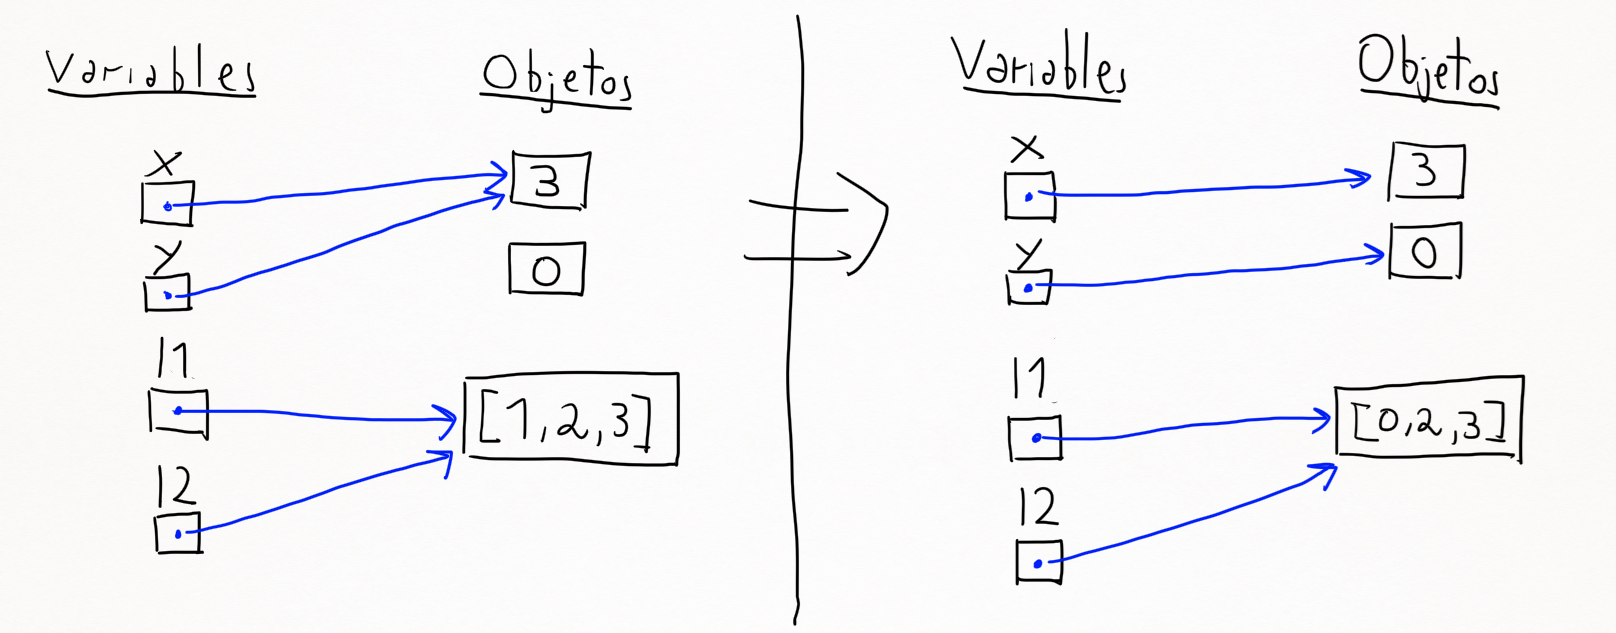
\includegraphics[scale=0.3]{ejemploVarMem.png}
	\caption{Ilustración de ejemplo presentado en la sección \ref{sec-memoriaCompartida}}
	\label{fig-ejemploVarMem}
\end{figure}

Los números son objetos {\bf inmutables}: no se pueden modificar. Las listas, por otra parte, son objetos {\bf mutables}, lo cual significa que pueden ser modificadas. Un ejemplo es cuando se modifica uno de sus elementos, como al ejecutar {\tt l2[0]=0}. Esta distinción de mutable o inmutable se aplica a los objetos de python en general. Los strings por ejemplo también son inmutables.



\section{Programas e instrucciones}

Digamos que programa en python es una secuencia de instrucciones que se almacena en un archivo de formato <<{\tt .py}>>. Un ejemplo básico de instrucción es la asignación, que ya vimos. Por otra parte, cuando escribimos una expresión o una variable en el intérprete y damos enter para que imprima el valor, también se trata de una instrucción. Estas últimas en general se usan solamente haciendo experimentos sencillos en el intérprete; no es común incluirlas en programas.

Al ejecutar un programa (ver figura \ref{fig-ejecPython}) se ejecutan las instrucciones en el orden que están escritas.

La siguiente lista contiene otros ejemplos de instrucciones que pueden ser útiles.
\begin{itemize}
	\item {\tt print()}. Se trata de una instrucción que imprime en la consola lo que se le pasa como parámetro. Es la instrucción por excelencia para mostrar algo en la consola. Si se le pasa un valor directamente imprime ese valor, mientras que si se le pasa una variable imprime el contenido de la variable. Por ejemplo, la instrucción {\tt print("Hola")} imprime <<Hola>>, mientras que {\tt print(x)} imprime el valor de la variable {\tt x} (y si esta variable no tiene ningún valor, da error).
	
	\item {\tt input()}. Se trata de una instrucción que permite leer algo que el usuario escriba en la terminal. Es una herramienta rudimentaria para hacer programas interactivos. Lo que se escribe entre paréntesis es un texto que se le muestra al usuario antes de esperar a que este escriba algo. La forma de uso es en general  {\tt x=input()}. De esta forma, lo que escriba el usuario se guarda como un string en la variable {\tt x}. En caso de ser necesario, se puede convertirlo a otro tipo de dato, como veremos en el ejemplo a continuación. Al llegar a una instrucción de este tipo, la ejecución del programa se detiene hasta que el usuario escriba algo y presione enter.
	
	\item {\tt append()}. Esta instrucción es para agregar un elemento al final de una lista. A diferencia de las anteriores, es formalmente lo que se llama un {\sl método} de las listas. Dada una lista {\tt l} y un objeto $x$ que queremos agregar al final, la instrucción es {\tt l.append($x$)}. Se escribe el nombre de la lista, un punto y luego {\tt append()} con lo que querramos agregar adentro de los paréntesis. 
	
	\item {\tt del}. Permite (entre otras cosas) quitar el elemento de cierto índice de una lista. Dada una lista {\tt l}, la instrucción {\tt del l[i]} quita el elemento de índice {\tt i}. Si hay elementos después del {\tt i}ésimo, sus índices se decrementan.
\end{itemize}

Existen muchas otras instrucciones en python, pero no es el foco del curso aprender una gran cantidad. En general hay muchas que hacen cosas que con un poco de trabajo se pueden realizar utilizando otras. Veamos un ejemplo de programa en el que se usan estás dos instrucciones de entrada/salida mencionadas.
\begin{verbatim}
print("Hola.")
x = input("Ingrese su numero favorito por favor: ")
print("Su numero favorito es " + x) #Notar que x es un string.
xNum = int(x) #Con esta instruccion, el string x se convierte en un entero.
print("El doble de su numero favorito es ", 2*xNum)
#Se puede imprimir mas de una cosa separando con comas.
\end{verbatim}
Estas líneas son el contenido de un archivo llamado <<ejemplo1.py>>. Al ejecutarlo en la terminal e ingresar <<5>> al momento del input, ocurre lo siguiente:
\begin{verbatim}
PS C:\Users...\Computación\Programas\ejemplo1> python ejemplo1.py
Hola.
Ingrese su número favorito por favor: 5
Su número favorito es 5
El doble de su número favorito es  10
\end{verbatim}
La ejecución del programa se detuvo después de mostrar <<{\tt Ingrese su número favorito por favor: }>>. Luego escribí <<5>>, presioné enter y ahí continuó. Si escribiera algo que no sea un entero válido, la operación {\tt int(x)} fallaría. En ese caso se imprime en la terminal una explicación del error y la ejecución se corta en ese punto.

Recomiendo ejecutar este ejemplo por uno mismo. Alcanza con copiar y pegar el código escrito arriba en un archivo y ejecutarlo.

\section{Condicionales}

Con lo que tenemos hasta ahora, la secuencia de instrucciones que se ejecuta en un programa es algo estático. Independientemente de lo que ocurra, las instrucciones se ejecutan de la primera hasta la última. Las instrucciones, por otra parte, permiten escribir código que se ejecute o no en función de cierta condición. La sintaxis es la siguiente:
\begin{lstlisting}[language=python]
if cond:
    code
\end{lstlisting}
Se escribe la palabra clave <<if>>, luego se escribe una condición, que es cualquier cosa que se evalue en algo de tipo booleano, luego se escribe un símbolo <<:>> y abajo, con una sangría de 4 espacios, se escribe el código que debe ejecutarse en caso de que la condición se cumpla. La sangría es muy importante, pues delimita lo que está sujeto a la condición. Ejemplifiquemos esto. En el siguiente código:
\begin{verbatim}
if cond:
    instr1
instr2
instr3
\end{verbatim}
en caso de que se cumpla {\tt cond}, se ejecuta {\tt instr1}. Después de eso, independientemente de la condición, se ejecutan {\tt instr2} e {\tt instr3}. Por otra parte, consideremos ahora:
\begin{verbatim}
if cond:
    instr1
    instr2
instr3
\end{verbatim}
En este caso, si se cumple {\tt cond}, entonces se ejecutan {\tt instr1} e {\tt instr2}. Después de eso, independientemente de la condición se ejecuta {\tt instr3}.

La instrucción {\tt if} se puede extender con más cosas. Estas extensiones no nos permiten hacer nada que no pudiéramos hacer solamente con ifs, pero ayudan a escribir código más claro. Por ejemplo, se puede agregar una cláusula {\tt else} para algo que se ejecute en caso de que no se cumpla la condición. Con esto la instrucción queda:
\begin{verbatim}
if cond:
    instr1
else:
    instr2
\end{verbatim}
De esta forma, si se cumple {\tt cond} se ejecuta {\tt instr1} y si no, se ejecuta {\tt instr2}. Es equivalente a:
\begin{verbatim}
if cond:
    instr1
if not cond:
    instr2
\end{verbatim}

La otra extensión común es con {\tt elif}. Esto es como un {\tt else if}. Es para poner algo que se haga en caso de que la condición anterior no se cumpla pero otra condición sí se cumpla. Después de un {\tt if} se pueden poner tantos {\tt elif} como se desee. Por ejemplo, podemos escribir
\begin{verbatim}
if cond1:
    instr1
elif cond2:
    instr2
elif cond3:
    instr3
else:
    instr4
\end{verbatim}
que es equivalente a:
\begin{verbatim}
if cond1:
    instr1
else:
    if cond2:
        instr2
    else:
        if cond3:
            instr3
        else:
            instr4
\end{verbatim}
Dicho sea de paso, se puede poner ifs adentro del cuerpo de otros ifs, como acabamos de hacer para escribir algo equivalente a los elif.

A modo de ejemplo, podemos escribir el siguiente programa que pide un entero al usuario y le dice si este entero es negativo, cero o positivo.
\begin{verbatim}
x = int(input("Ingrese un entero "))
#De una leemos lo que escribe el usuario y lo convertimos en un entero
if x < 0:
    print("El número es negativo")
elif x == 0:
    print("El númemro es cero")
else:
    print("El número es positivo")
print("Gracias.") #Esto siempre se ejecuta al final.
\end{verbatim}

\begin{ejercicio}
	Escribir la siguiente instrucción usando cuatro ifs seguidos (sin meter un if adentro del cuerpo de otro).
\begin{verbatim}
if cond1:
    instr1
elif cond2:
    instr2
elif cond3:
    instr3
else:
    instr4
\end{verbatim}

\end{ejercicio}

\section{Iteraciones}

Los distintos tipos de iteraciones son tal vez la herramienta más fuerte en la programación. Una computadora tiene la capacidad de ejecutar millones de instrucciones por segundo, pero escribir millones de instrucciones no es viable. La forma de aprovechar esta capacidad es con los ciclos, o iteraciones, que nos permiten decir a la computadora que repita algo muchas veces. De esta forma, con una cantidad razonable de lineas de código podemos hacer que la computadora ejecute muchas instrucciones. Veremos dos tipos de iteraciones, el {\tt for} y el {\tt while}.

El {\tt for} (en python) nos permite iterar a travez de los elementos de una lista y hacer algo con cada uno de ellos. La sintaxis es:
\begin{lstlisting}[language=python]
for x in lista:
    code
\end{lstlisting}
donde {\tt lista} es la lista a recorrer, {\tt x} es una variable nueva que irá recorriendo los elementos de esta lista y {\tt code} es el código que se ejecuta para cada elemento de la lista. Nuevamente la sangría del código es importante para delimitar las instrucciones que se iteran. Dentro del código se puede usar la variable {\tt x}, cuyo contenido va variando por los elementos de la lista de modo ordenado.

Si el contenido de la lista es $[a_1,a_2,\dots,a_n]$, entonces lo que ocurre es lo siguiente. Primero {\tt x} toma el valor $a_1$ y se ejecuta {\tt code}. Después {\tt x} toma el valor $a_2$ y se vuelve a ejecutar {\tt code}. Sigue así sucesivamente hasta que finalmente se ejecuta {\tt code} con {\tt x} valiendo $a_n$.

A modo de ejemplo:
\begin{verbatim}
lista = [1,2,3,4,5]
for x in lista:
    print(x)
print("Fin.")
\end{verbatim}
imprime los elementos de la lista en orden y luego un <<Fin.>>.

Una funcionalidad de python que se suele usar conjuntamente es la función {\tt range()}. Se puede pensar que {\tt range($n$)} es la lista de enteros que comienza en $0$ y termina en $n-1$. Internamente se representa distinto, pero conceptualmente es eso. Con dos parámetros se puede elegir también el comienzo. Los elementos de {\tt range($a,b$)} son los~$i$ tales que $a\leq i<b$. Esto nos permite por ejemplo escribir un programa que sume todos los números menores a cierto $n$.
\begin{verbatim}
n = int(input("Elija el n: "))
suma = 0
for i in range(n): #range(n) es [0,1,2,...,n-1]
    suma = suma + i
print(suma)
\end{verbatim}
\begin{ejercicio}
	Escribir un programa que pida dos entradas $a$ y $b$ y retorne la suma de todos los números $n$ tales que $a\leq n\leq b$. Notar que queremos incluir a $b$ en la suma. Luego de escribir el programa hacer algunas pruebas para ver si anda bien (una buena práctica que se suele llamar {\sl testing}). Recomiendo en general hacer pruebas, independientemente de que se pida en la letra o no.
\end{ejercicio}

Pasamos ahora a los ciclos {\tt while}. En este caso, el ciclo está definido por una condición booleana y se repite el contenido hasta que esta condición sea falsa. La sintaxis es:
\begin{lstlisting}[language=python]
while cond:
    code
\end{lstlisting}
donde {\tt cond} es algo que se evalúa a un valor booleano y {\tt code} es lo que queremos que se ejecute mientras la condición se cumpla.

La ejecución es como sigue. Primero se evalúa la condición. Si esta es falsa, termina la ejecución del while. Si es verdadera, se ejecuta {\tt code}, luego se vuelve a evaluar la condición y se vuelve a tomar la misma disyuntiva, así sucesivamente hasta que la condición sea falsa.

La iteración solo se detiene si la condición es falsa. En caso de que nunca se haga falsa, la ejecución entra en un bucle infinito.

El while es una herramienta muy poderosa, porque nos permite hacer iteraciones que a priori no sabemos la cantidad de veces que se van a ejecutar (en un for es el largo de la lista), pero introduce el riesgo de que nuestro programa no termine nunca. En la computación, esto es algo con lo que hay que convivir, prestando atención al escribir los programas.

Veamos un ejemplo que determina si un número $n\geq 2$ es primo o no. El razonamiento es el siguiente. Vamos a ir recorriendo números menores a $n$ para ver si encontramos un divisor. La idea es ir probando con números sucesivos hasta que encontremos un divisor o lleguemos a $n$.
\begin{verbatim}
n = int(input("Introduzca un entero mayor a 1: "))
puede_ser_primo = True
potencial_divisor = 2
while puede_ser_primo and potencial_divisor < n:
    if n % potencial_divisor == 0: #Es un divisor de n
        puede_ser_primo = False
    potencial_divisor = potencial_divisor + 1
if puede_ser_primo:
    print("Es primo")
else:
    print("No es primo")
\end{verbatim}
Podría hacerse también con un for, haciendo que se recorra todo {\tt range(2,n)} y para cada elemento se determine si es un divisor o no. La ventaja de hacerlo con el while es que una vez que encontramos un divisor, dejamos de iterar. Si por otra parte usamos el for, aunque en seguida encontraramos un divisor y ya sepamos que no es primo, seguiriamos iterando hasta llegar a $n-1$.
\begin{ejercicio}
	Escribir un programa para determinar si un número es primo que use for (independientemente de la desventaja que acabamos de mencionar).
\end{ejercicio}

Un uso de los while es el de hacer un programa que pueda repetirse tantas veces como el usuario quiera. Para esto lo que podemos hacer es:
\begin{verbatim}
continuar = True
while continuar:
   programa... #Aquí está el programa que debe repetirse
               #hasta que el usuario decida lo contrario
   respuesta = input("Si desea repetir ingrese 1, sino ingrese 0: ")
   if respuesta == 0:
       continuar = False
\end{verbatim}
\begin{ejercicio}
	Aplicar esto último con alguno de los programas que determinan si un número es primo.
\end{ejercicio}
\section{Funciones}

En programación se le llama función a un fragmento de código separado del resto que puede recibir parámetros y retornar valores. Proviene del concepto matemático de función. No permiten hacer nada que no se pudiera hacer con lo que ya vimos, pero son útiles para que los programas queden más fáciles de entender y para reutilizar código. Esto último es porque una función se define una sola vez y se puede utilizar fácilmente como parte de distintos programas. La sintaxis es la siguiente:
\begin{lstlisting}[language=python]
def nombre_fun(p_1,...,p_n):
    code	
\end{lstlisting}
Se escribe la palabra reservada {\tt def}, luego el nombre de la función, luego una secuencia de parámetros (cero o más), que son nombres de variables, luego un <<:>> y luego el código con sangría. En este código se puede usar la instrucción especial {\tt return} para que la función retorne un valor. La idea es que en términos matemáticos es una función que se aplica a los parámetros y su imagen es lo que se indica con {\tt return}. A modo de ejemplo, la función valor absoluto se puede escribir de la siguiente forma:
\begin{verbatim}
def val_abs(x):
    if x >= 0:
        return x
    else:
        return -x
\end{verbatim}
Si en un programa ponemos solamente la definición de la función y no escribimos nada más después, ese programa no hace nada. Por otra parte, después de la definición podemos ejecutarla en un argumento $x$ escribiendo {\tt val\_abs($x$)}. 

\begin{verbatim}
def val_abs(x):
    if x >= 0:
        return x
    else:
        return -x
valor1 = val_abs(0)
valor2 = val_abs(6)
valor3 = val_abs(-46)
print(valor1, valor2, valor3)
\end{verbatim}
Si se ejecuta este programa lo que se ve en consola es que imprime <<0 6 46>>. Notar que escribimos la función una vez y pudimos ejecutarla para tres argumentos distintos; en esto radica la utilidad de las funciones.

Si una función tiene varios parámetros, al ejecutarla el orden de los argumentos es el mismo. Por ejemplo, si escribimos una función {\tt f(x,y)} y luego ejecutamos {\tt f(1,2)}, entonces {\tt x} será 1 y {\tt y} será 2.

Hagamos un ejemplo un poco más complejo vinculado con números primos. A partir del código que ya hicimos en la sección de iteraciones podemos escribir una función que reciba como parámetro un número y retorne un booleano que diga si es primo o no.
\begin{verbatim}
def es_primo(n):
    if n<2:
        return False
    puede_ser_primo = True
    potencial_divisor = 2
    while puede_ser_primo and potencial_divisor < n:
        if n % potencial_divisor == 0: #Es un divisor de n
            puede_ser_primo = False
        potencial_divisor = potencial_divisor + 1
    return puede_ser_primo
\end{verbatim}
Cabe aclarar que cuando se ejecuta un {\tt return} la función termina, independientemente de que después haya más código o no. Veamos varios ejemplos de usos para esta función. Primero, para hacer lo mismo que antes alcanza con después escribir:
\begin{verbatim}
n = int(input("Introduzca un entero mayor a 1: "))
if es_primo(n):
    print("Es primo")
else:
    print("No es primo")
\end{verbatim}
Por otra parte, podemos hacer una función que pida dos números e imprima todos los primos comprendidos entre ellos.
\begin{verbatim}
min = int(input("Introduzca el extremo inferior: "))
max = int(input("Introduzca el extremo superior: "))
for n in range(min, max+1): #Incluyo max
    if es_primo(n):
        print(n, end=",") #Lo de end es para que queden en la misma línea
                          #separados por comas
\end{verbatim}
Por último escribamos un programa que dado un $n$ nos diga cual es el primer primo mayor a $n$. Como los primos son infinitos, sabemos que el programa termina para cualquier entrada.
\begin{verbatim}
n = int(input("Introduzca un entero: "))
while not es_primo(n):
    n = n + 1
print("El mínimo primo mayor o igual es ", n)
\end{verbatim}
Notar como dato interesante que la terminación de este programa para cada entrada es de hecho equivalente a la existencia de infinitos primos. La cuestión de si un programa termina o no puede un problema difícil. No siempre se puede resolver empíricamente, sino que en general hay que hacer una demostración. El motivo de esto es que si lleva mucho tiempo sin terminar, no tenemos forma de saber si es que no va a terminar nunca o que sí va a terminar pero más adelante.

Una función puede no tener parámetros y también puede no retornar nada. En los casos en los que no retorna nada (simplemente hace ciertas cosas), lo cual se aparta mucho del concepto matemático de función, en algunos lenguajes se les llama procedimientos. En python se les llama igual funciones porque en realidad retornan un valor trivial que no se muestra (detalle formal). Un ejemplo de función que no tiene parámetros ni retorna nada sería:
\begin{verbatim}
def bienvenida():
    t = input("Hola, ¿cómo te llamas? ")
    print("Bienvenid@, ",t)
\end{verbatim}
Se trata de una función que le da la bienvenida al usuario. Dentro de un programa podría ejecutarse al principio, poniendo <<{\tt bienvenida()}>> como primera línea y no afectaría en nada para el resto del programa.

\subsection{Variables locales y globales}
Veamos un par de detalles técnicos sobre nombres de variables y funciones. Primero, las variables que se definen dentro de una función se llaman {\bf locales} y solo están definidas dentro del cuerpo de la función. Esto es para que el funcionamiento interno de la función sea bastante independiente al resto del código. En general la idea es que la función interactúa con el resto del programa solamente (o principalmente) mediante los parámetros y el valor que retorna. Veamos un ejemplo.
\begin{verbatim}
def f(n):
    x = 10
    return n + x
y = f(3)
print(x) #Esto da error porque x solo está definida adentro de la función
\end{verbatim}

Por otra parte, las variables que se definen antes de la definición de la función pueden usarse dentro de esta y también siguen definidas después. A estas variables se les llama {\bf globales}. Por ejemplo:
\begin{verbatim}
x = 10
def f(n):
    return n + x #Usamos la variable x definida antes
y = f(3)
print(x) #Ahora acá no da error
\end{verbatim}
Sin embargo, este comportamiento se da si solamente leemos el contenido de la variable sin modificarla. En caso de que hagamos una asignación a {\tt x}, no la realizará con la variable global, sino que creará una variable local con el mismo nombre que dentro de la función remplazará a la variable global. Por lo tanto, los cambios que se hagan no se reflejarán afuera. Por ejemplo:
\begin{verbatim}
x = 5 #Variable global
def f(n):
    x= 10 #Asigna 10 a una nueva variable local sin modificar la global
    return n + x #Acá x es la variable local, no la global
y = f(3) #el valor de f(3) es 13
print(x) #Imprime 5, que es el valor de la variable global
\end{verbatim}

Por último, una función que se define antes que otra puede usarse en la segunda. El vínculo de esto con lo que venimos viendo es que el nombre de la primera función es como una variable global para la segunda.
\begin{verbatim}
def f1(n):
    return n + 5
def f2(x):
    return 5*f1(x)
\end{verbatim}

\section{Metodología de resolución de problemas}

Cuando tenemos un problema complejo no suele ser una buena idea ir directamente a programar. De hecho, en general el desarrollo de software tiene muchas etapas, en varias de las cuales no se programa. Veamos una metodología sencilla, la cual se recomienda usar para resolver problemas en el curso. De hecho, de modo más abstracto puede ser útil para resolver problemas en general, no necesariamente de programación. La metodología consta de cuatro etapas: análisis, diseño, implementación y verificación.
\begin{itemize}
	\item Análisis. Se trata de estudiar el problema a resolver, asegurándose de entender qué es exactamente lo que se debe hacer. Es importante entender los conceptos y definiciones pertinentes al contexto donde está el problema. Esta etapa puede ser de las más complejas en aplicaciones de software en la vida real. Imaginarse por un momento hacer un programa para ser usado en medicina; primero habría que entender qué cosas se hacen exactamente, junto con mucha terminología específica del rubro. En problemas como los que veremos en el curso no suele hacer falta mucho trabajo en esta etapa, pero si no se hace correctamente (o sea, si no se entiende bien lo que se debe hacer), independientemente del esfuerzo que se haga después, el resultado no será correcto.
	
	\item Diseño. Se trata de diseñar una solución al problema, pensando a grandes rasgos la estrategia que se utilizará, sin meterse aún a programar nada. En general la estrategia incluye descomponer al problema como una secuencia de subproblemas más fáciles.
	
	\item Implementación. Se programa la solución al problema, siguiendo la estrategia que se definió en la etapa de diseño.
	
	\item Verificación. Es común que se use la palabra en inglés: {\sl testing}. Se hacen pruebas para verificar si la solución tiene el comportamiento esperado. No se trata de una demostración formal de que el programa funciona, sino que de experimentos puntuales que aseguran solamente que el programa funciona en ciertos casos. La verificación no es infalible, pero si se hace bien, hay buenas chances de que en caso de que haya un error lo detectemos, así que es recomendable hacerlo.
\end{itemize}

Claramente el análisis y el diseño deben ser lo primero que se hace. Por otra parte, cuando la estrategia tiene varias etapas, es recomendable ir intercalando implementación y verificación, es decir, escribir una parte del programa, hacer pruebas para ver si está bien (en caso de que hayan errores corregirlos) y recién después de tener cierta certeza de esto, pasar a la siguiente etapa.

Para la verificación se pueden hacer casos concretos ingresados a mano o un programa que chequee automáticamente muchos casos para los que sabemos la respuesta. En el ejemplo que viene ahora haremos ambas cosas (y hay un ejercicio de esto en el práctico 1, titulado {\sl testing automático}).

\subsection{Ejemplo}

Veamos un ejemplo (bastante artificial), para le cual aplicaremos la metodología. Supongamos que un cliente nos pide un programa que resuelve el siguiente problema.

{\it Sea {\tt l} una lista de enteros positivos. Determinar si la cantidad de números $n\in\mathtt{l}$ tales que su cantidad de dígitos también está en {\tt l} es un número primo.}

{\bf Análisis}. Hay que asegurarnos de entender bien lo que se pide. En caso de que algo no esté claro, habría que consultar al cliente (salvo que sea evidente que sea irrelevante). Después de haber leído {\sl bien} la consigna, puede ser una  buena idea pensar en algunos ejemplos. La lista {\tt [10,11,12,2]} cumple la propiedad, porque la cantidad es $3$, mientras que la lista {\tt [1,2,3,4]} no la cumple, porque la cantidad es $1$. Que en la segunda lista sea $1$ es porque la cantidad de dígitos de $1$ es $1$ mismo, el cual está en la lista. Sin embargo, esta característica de $1$ ¿será la idea considerarlo o no? Por otra parte, a priori la lista podría tener números repetidos. ¿En ese caso los contamos varias veces o no? Hacemos las preguntas al cliente y nos responde lo siguiente.

{\it Primero, está bien que $1$ cuente. Segundo, de hecho la lista no tiene números repetidos.}

Ahora que resolvimos esas dudas, parece ser una buena idea pasar a la siguiente etapa, aunque si llegáramos a darnos cuenta de algún otro detalle, podríamos volver a preguntarle al cliente.

{\bf Diseño}. La idea es determinar subproblemas más sencillos tales que si los resolvemos a todos, tenemos una solución al problema original. Por ejemplo, podemos considerar los siguientes:
\begin{enumerate}
	\item Determinar la cantidad de dígitos de un número.
	\item Determinar si un número está en una lista.
	\item Determinar si un número es primo.
\end{enumerate}
Juntando los items 1 y 2, podemos determinar si la cantidad de dígitos de un número está en la lista. Podemos entonces iterar a lo largo de la lista y para cada número determinar si su cantidad de dígitos está o no, llevando la cuenta de cuántos son. Finalmente, determinamos si ese número es primo.

{\bf Implementación y verificación}. Escribamos funciones para cada una de los tres items de arriba. Después de cada función, haremos algo de verificación antes de continuar. Para la parte de determinar si un número es primo usamos la función que ya tenemos de antes.

\begin{verbatim}
	def es_primo(n):
	    if n<2:
	        return False
	    puede_ser_primo = True
	    potencial_divisor = 2
	    while puede_ser_primo and potencial_divisor < n:
	        if n % potencial_divisor == 0: #Es un divisor de n
	            puede_ser_primo = False
	        potencial_divisor = potencial_divisor + 1
	    return puede_ser_primo
\end{verbatim}

Ingresamos esta función en un archivo llamado {\tt programa.py} y hacemos algunas pruebas desde la terminal.
\begin{verbatim}
PS C:\Users\...\Ejemplo metodología> python -i programa.py
>>> es_primo(1)
False
>>> es_primo(2)
True
>>> es_primo(3)
True
>>> es_primo(4)
False
>>> es_primo(5)
True
>>> es_primo(12)
False
>>> es_primo(41)
True
>>> es_primo(49)
False
\end{verbatim}
Hasta ahí parece estar andando bien. Para pruebas automáticas podríamos ver por ejemplo si para todos los pares entre $4$ y $100$ retorna falso. Escribimos por ejemplo el siguiente programa.
\begin{verbatim}
pasa_test = True
for i in range(2,101):
    if es_primo(2*i):
        pasa_test = False
if pasa_test:
    print("Pasa el test")
else:
    print("No pasa el test.")
\end{verbatim}
Agregamos ese programa al final del archivo {\tt programa.py} y lo ejecutamos. Obtenemos la siguiente salida.
\begin{verbatim}
PS C:\Users\...\Ejemplo metodología> python programa.py
Pasa el test
\end{verbatim}
Por lo tanto, el test fue satisfactorio. Nos quedamos conformes con esto y seguimos con el resto (qué tanto testing hacer es a decisión de cada uno). Borramos del archivo {\tt programa.py} este caso de prueba, o lo guardamos en otro archivo distinto.

Escribamos ahora una función para determinar la cantidad de dígitos de un número. Podemos hacer lo siguiente.
\begin{verbatim}
# la entrada es un entero positivo.
# retorna la cantidad de dígitos del número escrito en base 10.
def cant_digitos(n):
    cant = 1
    q = n // 10
    while q > 0:
        cant = cant + 1
        q = q // 10
    return cant
\end{verbatim}
Notar que arriba de la función escribimos un comentario que aclara lo que hace. Esto es una muy buena práctica que se recomienda aplicar en general (aunque aquí lo hacemos solo con esta función). Si bien ahora tenemos claro lo que hace, si volvemos a mirar la función dentro de un tiempo, el comentario nos vendrá muy bien. Agregamos esta función al archivo {\tt programa.py} y hacemos pruebas del mismo modo que con la función anterior. Hacemos algunas pruebas a mano. Para testing automático podemos verificar por ejemplo que para cada $a$ entre $1$ y $9$ y para cada $n$ menor a $100$, la función retorna $n+1$.
\begin{verbatim}
pasa_test = True
for a in range(1,10):
    for n in range(100):
        if cant_digitos(a*10**n) != n+1:
            pasa_test = False
if pasa_test:
    print("Pasa el test")
else:
    print("No pasa el test.")
\end{verbatim}
Verificamos que se pasa el test y continuamos con la siguiente. Vamos a escribir una función que diga si un número está en una lista.
\begin{verbatim}
def pertenece(n,l):
    for i in l:
        if i == n:
            return True
    return False #Si llega acá es porque no está
\end{verbatim}
Queda como ejercicio hacer un poco de testing para esta función.

Finalmente, usando lo anterior como dijimos en la etapa de diseño podemos escribir una función que resuelva el problema.
\begin{verbatim}
def problema(l):
    cant = 0
    for n in l:
        if pertenece(cant_digitos(n),l):
            cant = cant + 1
    return es_primo(cant)
\end{verbatim}
Notar que al haber separado el problema en subproblemas, la función final quedó muy sencilla. Finalmente el contenido del archivo {\tt programa.py} es:

\begin{verbatim}
def es_primo(n):
    if n<2:
        return False
    puede_ser_primo = True
    potencial_divisor = 2
    while puede_ser_primo and potencial_divisor < n:
        if n % potencial_divisor == 0: #Es un divisor de n
            puede_ser_primo = False
        potencial_divisor = potencial_divisor + 1
    return puede_ser_primo
# la entrada es un entero positivo.
# retorna la cantidad de dígitos del número escrito en base 10.
def cant_digitos(n):
    cant = 1
    q = n // 10
    while q > 0:
        cant = cant + 1
        q = q // 10
    return cant

def pertenece(n,l):
    for i in l:
        if i == n:
            return True
    return False #Si llega acá es porque no está

def problema(l):
    cant = 0
    for n in l:
        if pertenece(cant_digitos(n),l):
            cant = cant + 1
    return es_primo(cant)
\end{verbatim}

Lo siguiente son algunas pruebas.
\begin{verbatim}
PS C:\Users\...\Ejemplo metodología> python -i programa.py
>>> l = [1,2,3] 
>>> problema(l) #Hay 3
True
>>> l.append(4)
>>> problema(l) # Hay 4
False
>>> l.append(10) # Hay 5
>>> problema(l)
True
>>> l.append(123123123) 
>>> problema(l) #El número nuevo no afecta
True
\end{verbatim}
Queda como ejercicio para quien quiera hacer pruebas automatizadas. Si fuera un problema real claramente habría que verificar bien a la función final.

Respecto a la función {\tt pertenece(n,l)}, si bien para este ejemplo escribimos una función, de hecho en python escribir {\tt n in l} tiene el mismo resultado. Es decir, {\tt in} es un operador que dado un objeto y una lista retorna el booleano que indica si pertenece o no.
\end{document}


